
We formulate the problem of generating colorings for a pattern template as finding high-probability colorings under a probabilistic model. Formally, we define a pattern template as $\pattern = (\segments, \groups, \colorVars, \features)$, where $\groups$ is a set of individual groups $\group$, and $\segments$ is a set of individual segments $\segment$, $\colorVars$ is a set of color variables, and $\features$ is a set of features over different groups, segments, and segment adjacencies within the pattern. Each $\group$ and $\segment$ is associated with a color variable ($\colorVars_\group$ and $\colorVars_\segment$, respectively). All segments within a color group have the same color by definition, so $\colorVars_{\text{group}(\segment))} = \colorVars_\segment$. A coloring $\colors$ is an assignment of colors to color variables.

We define the probability of a coloring for a particular pattern template as a log-linear model~\cite{LogLinearModels}:  
\begin{equation*}
 p(\colors | \pattern : \weights) = \frac{1}{Z_\pattern(\weights)} \prod_{\term \in \model} \exp{\frac{ \weights_\term \cdot \termStats(\colors, \pattern)}{t}}
\end{equation*}
The model $\model$ is comprised of a number of different terms $\term$, where each term scores the goodness of a color assignment based on a term-dependent sufficient statistics function $\termStats(\colors,\pattern)$. $Z_\pattern(\weights)$ is the pattern-dependent partition function that normalizes the distribution. The temperature $t$ affects the peakiness of the distribution and will play a role in sampling from the model, as described in Section~\ref{sec:sampling}. Each term also has a weight $\weights_\term$ which determines its relative contribution to the model; the method used for setting these weights is detailed in Section~\ref{sec:weights}.

This type of model is well-suited to the coloring-generation problem. It is very flexible; in principle, the individual term statistics $\termStats$ can be any real-valued function. In our model, we include terms both for color compatibility as well as for spatial properties defined over groups, segments, and segment adjacencies. Users can also guide the model via additional soft constraint terms (Section~\ref{sec:results}). In addition, it is very easy to compare the relative importance of each term by comparing their weights, which we will do in Section~\ref{sec:weights} to gain some insight into which terms contribute the most to producing attractive colorings. 

The model can also be interpreted graphically as a factor graph~\cite{FactorGraphs}. Each type of term contributes different factors to the graph. For example, the color compatibility term contributes a factor touching at most five color variables that scores the compatibility of those colors. The spatial terms contribute a unary factor for each color variable and binary factors for color variables that are adjacent in the pattern. Figure~\ref{fig:FactorGraph} shows an example of such a factor graph. Circles denote the color variables, while squares denote the different factors $\factor$, and edges connect each factor to the variables within their scope. 


\begin{figure}[ht]
\begin{tabular}{cc}
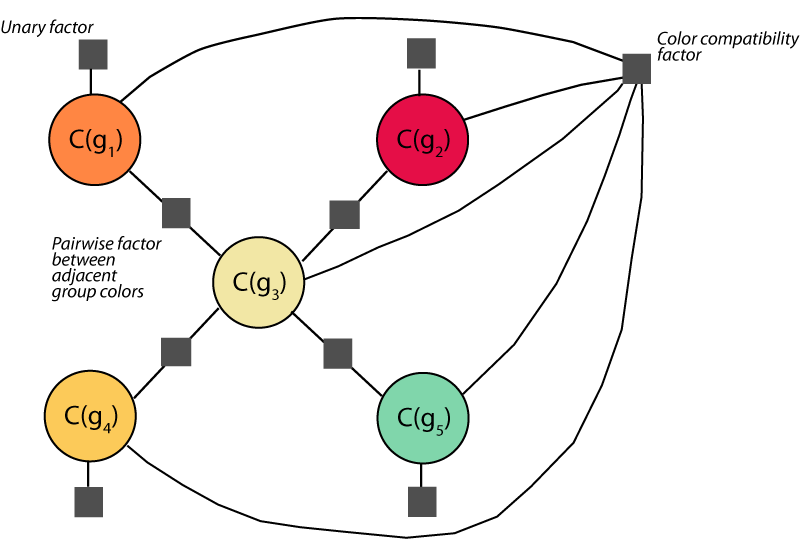
\includegraphics[width=.7\columnwidth]{figs/factorGraph} & 
\includegraphics[width=.2\columnwidth]{figs/factorGraphPattern}\\
\end{tabular} 
\caption{A factor graph for an example pattern template. Factors correspond with the color compatibility and spatial terms from our model. In the figure, nodes are colored according to their corresponding color group in the pattern\remark{Rough figure.}}
\label{fig:FactorGraph}
\end{figure}



\subsection{Color Compatibility}
\label{sec:colorCompat}

Previous work has shown that the aesthetic appeal of an image can be improved by increasing the compatibility or harmony of image colors ~\cite{CohenOrHarmonization,DressUp,ColorizationUsingHarmony,ODonovan}. Our model includes a color compatibility term to score the general appeal of the colors in an assignment, based on the compatibility model introduced by O'Donovan et al.~\shortcite{ODonovan}. This compatibility model predicts 0-5 numeric aesthetic ratings for five-color `color themes,' which are ordered rows of five colors. 

We extract such a color theme from a pattern by taking the colors of the five largest color groups and ordering them by size. If the pattern contains fewer than five color groups, we repeat colors in order of size to fill the rest of theme. Inspection of five-color patterns showed that size-ordering of colors tends to produce themes that are, on average, rated higher than random orderings but lower than the optimal ordering. Additionally, ordering has little effect on discriminative power: in general, low-scoring themes are rated lower than high-scoring themes regardless of permutation.

The term statistics function is then defined as the log-normalized theme rating under O'Donovan's compatibility model. Formally:
\begin{equation*}
\colorCompatTerm(\colors| \pattern) = \ln(\textrm{compat}(\textrm{theme}(\colors| \pattern))/5)
\end{equation*}
where $\textsl{theme}$ is the ordered theme extracted from the pattern and $\textsl{compat}$ is the predicted rating from the O'Donovan model.

Note that there is nothing special about the O'Donovan model that makes it work in our case. Our modeling framework is general enough to accomodate any color compatibility or harmony model that can `score' a set of colors.

In the factor graph representation of our model, this term contributes one factor that touches the five color variables belong to the five largest groups (or fewer, if there are less than five groups in the pattern). Formally:
\begin{equation*}
\factor(\textrm{top}(\colorVars) | \pattern) = \exp(\colorCompatWeight \cdot \colorCompatTerm(\colorVars | \pattern) / t)
\end{equation*}
where $\textsl{top}$ are the color variables of the largest five groups in the pattern, and $t$ is the temperature of the model as defined previously.

%\remark{S: Another possibility is to just define the factor sufficient statistics (need to find a good symbol for it), and then we don't need to keep writing the exp notation (with the temperature). Not sure if that would be more confusing. }

%\remark{S: To get more justification for the ordering criteria, we can also try looking at the ordered themes associated patterns and see if they look reasonable. I think we can also try getting the optimal rating of the top 5 colors in MATLAB (instead of having Scala pass permutations 120 times to MATLAB) to see how slow it is...or for comparison}.


\subsection{Spatial Properties}
\label{sec:spatialCompat}

As shown in Figure~\ref{fig:ColorCompatOnly}, color compatibility alone does not predict attractive colorings. Good color assignments also depend on the properties of the regions being colored and their spatial arrangement. To capture these dependencies, our model includes spatial terms over groups, segments, and segment adjacencies. Group and segment terms capture color dependencies on region features, and segment adjacency terms capture color dependencies on the relationship between nearby regions.

These spatial terms score color assignments based on the conditional probability of a color property $\prop$ (e.g. lightness or colorfulness) given the features of an object $x$ (which is either a group, segment, or segment adjacency). Formally:
%%
\begin{align*}
	\termStats(\colors | \pattern) &= \sum_{x \in \pattern} \termInstStats(\colors_x | \pattern, x) \\
	%\termInstStats(x, \colors| \pattern) &= \ln p(\prop(\colors(x)) | \features(x)) \cdot s_x
	\termInstStats(\colors_x | \pattern, x) &\propto p(\prop(\colors_x) | \features_x)
\end{align*}
%%
We compute these probabilities on color properties instead of directly on colors to allow for more generalization over colors that do not occur in the model's training data.
%$s_x$ is the contribution of $x$ to the overall score, and is based on the impact $x$ has on the appearance of the pattern (i.e. the area of a group or segment or the strength of an adjacency).

In the next sections, we give definitions for the group and segment terms in the model (Section~\ref{sec:groupAndSegTerms}) and the adjacency terms (Section~\ref{sec:adjTerms}). We then describe how to learn these terms from example patterns (Section~\ref{sec:learningPdfs}).

\subsubsection{Group and Segment Terms}
\label{sec:groupAndSegTerms}

Both global group features as well as local segment features affect the appearance of a color assignment. The total area of a group and overall spread of its member segments correspond to the overall proportion and spread of its assigned color within an image. In addition, the size and shape of member segments may impact the color a group takes on. As an example, smaller segments may often be more saturated, and a group composed of many small segments may be more likely to be saturated than a group composed of a few small segments but also one large segment \remark{S: Made up example. Should probably find one that holds in our data}.

Our model has one group and one segment term for each of the color properties $ \prop \in \unaryProps$, which is defined as
%%
\begin{align*}
\unaryProps = \{ &\propName{Lightness}, \propName{Colorfulness}, \\
                 &\propName{NameCounts}, \propName{NameSaliency} \}
\end{align*}
%%   
The properties \propName{Lightness} and \propName{Colorfulness} are computed in \lab space, a perception-based color space. \propName{NameCounts} (counts of how many times a color is described with different names) and \propName{NameSaliency} (how uniquely a color is named) are as described by Heer and Stone~\shortcite{ColorNamingModels}. While lightness and colorfulness capture perceptual properties of color, name saliency and color name counts capture more categorical properties. More details on the computation of these color properties can be found in the Appendix.

The group term for property $\prop \in \unaryProps$ has the sufficient statistics function:
\begin{align*}
 \groupTerm(\colors|\pattern) &= \sum_{\group \in \groups} \groupInstStats(\colors_\group | \pattern, \group) \\
 \groupInstStats(\colors_\group | \pattern, \group) &=  \ln p( \prop( \colors_\group ) | \features_\group ) \cdot \size_\group
\end{align*}
where $\size_\group$ is the size of the group $\group$ and $\features_\group$ are the features of the group $\group$ (See the Appendix for the complete list of features used). We weight the contribution of each group to the term statistics by its relative area as larger regions tend to have more impact on the appearance of a coloring.

Similarly, the segment term for property $\prop$ has the statistics function:
\begin{align*}
 \segTerm(\colors|\pattern) = \sum_{\segment \in \segments} \segInstStats(\colors_\segment | \pattern, \segment) \\
 \segInstStats(\colors_\segment | \pattern, \segment) = \ln p( \prop( \colors_\segment ) | \features_\segment) \cdot \size_\segment
\end{align*}
where $\size_\segment$ is the size of the segment $\segment$ and $\features_\segment$ are the features of $\segment$.

These terms contribute unary factors over each color variable by grouping together statistics for the group and segments associated with the variable. Formally:
\begin{align*}
 %\factor(\colorVars(\group)) = \prod_{\prop \in \unaryProps} \exp\left(\frac{\groupTermWeight \cdot \groupInstStats(\group) + \segTermWeight \cdot \sum_{\segment \in \group} \segInstStats(\segment)}{t}\right) 
 \factor(\colorVars_\group | \pattern) = \prod_{\prop \in \unaryProps}
 		\exp( (&\groupTermWeight \cdot \groupInstStats(\colorVars_\group | \pattern, \group)  \\
 		     + &\segTermWeight \cdot \sum_{\segment \in \group} \segInstStats(\colorVars_\group | \pattern, \segment)) / t) 
\end{align*}


\subsubsection{Segment Adjacency Terms}
\label{sec:adjTerms}

While group and segment terms model the dependency of color assignments on features of same-color regions, they do not capture relationships between different-color regions. In particular, adjacent color regions can have strong effects on their neighbor's perceived color, making colors seem more or less saturated or causing vibrating boundaries if adjacent lightness and colorfulness are too similar~\cite{AlbersInteractionOfColor}. Thus, we also add segment adjacency terms to the model.

Good color assignments to adjacent segments may depend on the nature of their adjacency. For example, a square enclosed by a thin border appears different from a square enclosed by a larger square, and different again from a square side-by-side with another square (Figure~\ref{fig:surround}). Thus, when computing features of an adjacency we include the features of the segments involved as well as how much one neighbor encloses another.
\begin{figure}[ht]
\centering

\includegraphics[width=.7\columnwidth]{figs/surround}
\caption{Color appearance depends on relationships with surrounding regions\remark{Rough figure.}}
\label{fig:surround}
\end{figure}



%~\remark{D: These examples might work better with pictures...} 

Our model has one adjacency term for each of the color properties $ \prop \in \binaryProps$, which is defined as
%%
\begin{align*}
\binaryProps = \{ &\propName{RelativeLightness}, \propName{RelativeColorfulness}, \\
                  &\propName{PerceptualDifference}, \propName{ChromaDifference}, \\
                  &\propName{NameSimilarity} \}
\end{align*}
%%
As with group and segment terms, \propName{RelativeLightness} and \propName{RelativeColorfulness} are computed in \lab space. \propName{PerceptualDifference} is Euclidean distance in \lab space, and \propName{ChromaDifference} is the percentage of that distance that is due to the chroma channels. Finally, \propName{NameSimilarity} is the color name cosine similarity measure defined by Heer and Stone~\shortcite{ColorNamingModels}.

The sufficient statistics function for each binary property is:
 \begin{align*}
 \adjTerm(\colors | \pattern) &= \sum_{(\segment, \segprime) \in \adj(\pattern)} \adjInstStats(\colors_\segment, \colors_\segprime | \pattern, \segment, \segprime) \\
 \adjInstStats(\colors_\segment, \colors_\segprime | \pattern, \segment, \segprime) &= \ln p( \prop( \colors_\segment, \colors_\segprime ) | \features_{\segment, \segprime} ) \cdot \adjStrength(\segment, \segprime)
\end{align*}
where $\adjStrength(\segment,\segprime)$ is the strength of the adjacency $(\segment,\segprime)$. We define adjacency strength as the number of pixels from segments $\segment$ or $\segprime$ that are within a 2-pixel distance from their perimeters. All adjacency strengths are normalized to sum to 1.  

These terms contribute binary factors over each adjacent pair of color variables:
\begin{equation*}
 %\factor(\colorVars(\group), \colorVars(\groupprime)) = \prod_{\prop \in \binaryProps} \exp\left(\frac{\adjTermWeight \cdot \sum_{(\segment, \segprime) \in \adj(\group, \groupprime)} \adjInstStats(\segment, \segprime)}{t}\right) 
 \factor(\colorVars_\group, \colorVars_\groupprime | \pattern) = \prod_{\prop \in \binaryProps} \exp( (\adjTermWeight \cdot \sum_{(\segment, \segprime) \in \adj(\group, \groupprime)} \adjInstStats( \colorVars_\group, \colorVars_\groupprime | \pattern, \segment, \segprime)) / t) 
\end{equation*}
%  \begin{equation*}
%  \factor(\colorVars(\group), \colorVars(\groupprime)) = exp\left(\sum_{\substack{\prop \in \binaryProps \\ (\segment, \segprime) \in \adj(\group, \groupprime)}} \adjTermWeight \cdot \adjInstStats(\segment, \segprime)\right) 
% \end{equation*}

\subsubsection{Learning Conditional Probability Distributions}
\label{sec:learningPdfs}

Each group, segment, and adjacency term requires a conditional probability distribution $p(\prop(\colorVars_x)|\features_x)$ in order to compute its statistics. What form should these distributions take? Closed-form continuous distributions, such as the normal distribution, are appealing for their simplicity.  However, they are unlikely to capture the nuances of data drawn from real patterns, which is often \emph{multimodal} in nature. As a simple example, pattern backgrounds are typically either very dark or very light. A normal distribution, which concentrates its probability mass at one mode, cannot faithfully capture this type of bimodal behavior.

In our model, we adapt the approach of Charpiat et al.~\shortcite{MultimodalColorization}, who learn conditional probability distributions of colors given local texture features for the purpose of grayscale image colorization. This method was designed explicitly to account for multimodality. The basic idea of our approach is as follows: first, the space of property values is discretized into a finite number of bins. Next, a regressor is trained on pairs of the form $(\prop(\colors_x), \features_x)$ to predict, given a feature vector $\features_x$, the probability that its corresponding property value $\prop(\colors_x)$ falls into each bin. Given a new, never-before-seen feature vector, the regressor can then output a histogram of these probabilities for each bin. The resulting histogram is then smoothed using a form of kernel density estimation, and the resulting density forms the final conditional probability distribution. Figure~\ref{fig:histograms} shows an example of raw and smoothed histograms for the background region of a pattern template (highlighted in orange).

We discretize the space of property values using K-means clustering on the values found in the training examples. The optimal number of bins is computed for each term using cross-validation.~\remark{Will this be true, in the final version of thigs?} We then use multinomial logistic regression to predict the histograms of property values given features. To ensure each pattern template in the training set has equal weight in the regression, we weight each group example by one over the number of groups in the template; segment and adjacency examples are weighted similarly. Finally, we smooth the histograms using the approach of Wang et al.~\shortcite{ThemeEnhancement}, which places a Gaussian at the center of each histogram bin. To set the Gaussian bandwidth, we use the average distance to the nearest three other bins.

\begin{figure}[ht]
\begin{tabular}{cc}
\raisebox{10em}{
\includegraphics[width=.22\columnwidth]{figs/histogramImage}}&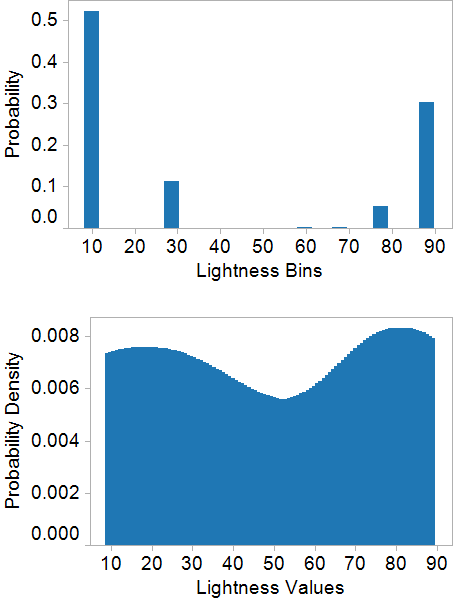
\includegraphics[width=.7\columnwidth]{figs/histograms}\vspace{0.5em}\\
\end{tabular}
\caption{Predicted histograms over lightness (right) for the background region of a pattern template (left). The region is highlighted in orange. The top histogram shows the discrete probability distribution over lightness bins (K=7), outputted by our regressors. The bottom histogram shows the probability density over lightness values after smoothing the discrete distribution.}
\label{fig:histograms}
\end{figure}



%\remark{D: This is a lot of abstract concepts. We really should have a figure, something from our Tableau visualizations, that shows e.g. a group and the predicted (smoothed) histogram.}

%However, we use multinomial logistic regression to predict the probability of a bin given a feature vector for an instance, instead of kernel density estimation on training instances that fall in the same bin. 
%
%TODO: multinomial logistic regression instead of KDE+KNN because....advantage of not having to store training instances, faster at inference time (though a bit slower at training time), and performance seemed reasonable qualitatively (or, was no worse than KNN). In addition, inspecting coefficients could be informative.  

%This approach is relatively fast. Because the features of a pattern template do not change during inference, we only need to compute the discretized conditional pdfs once per tuple of group, segment, or adjacency and their associated property when generating a coloring.~\remark{D: \emph{I} know what you mean, but I think readers would find this hard to parse. Maybe take a couple more sentences to make this clear?}